\documentclass[t]{beamer}
\usepackage{listings}
\usepackage{minted}

\usetheme{default}
\usebackgroundtemplate{
\includegraphics[width=\paperwidth]
                                       {../cpeb_bkground_topleftlogo.pdf}}

\setbeamertemplate{frametitle}{
  \centering\vspace{1mm}\insertframetitle\par\vspace{3mm}
}

\usepackage[style=nature,
            hyperref,
            backend=biber,
            isbn=false,
            doi=false,
            url=false,
            date=year,
            maxbibnames=3
           ]{biblatex}

\bibliography{KDM-kwip-tuebingen.bib}

\title{\texttt{kWIP}: The k-mer Weighted Inner Product}
\author{Kevin Murray}
\institute{Borevitz Lab, CPEB, ANU}
\date{25 Jan 2016}

\usefonttheme{serif}

\begin{document}

{
\usebackgroundtemplate{
\includegraphics[width=\paperwidth]{../cpeb_bkground_centered.pdf}}
\begin{frame}
  \titlepage
  \vfill
\end{frame}
}

\begin{frame}{\texttt{whoami}}
  \begin{columns}[t]
    \column{0.5\textwidth}
      \begin{itemize}
        \item PhD Student (Bioinformatics)
        \item ``Novel algorithms for plant population genomics''
      \end{itemize}
    \column{0.5\textwidth}
      \begin{itemize}
        \item Justin Borevitz Lab, ANU
        \item Canberra, Australia
      \end{itemize}
  \end{columns}
  \begin{center}
    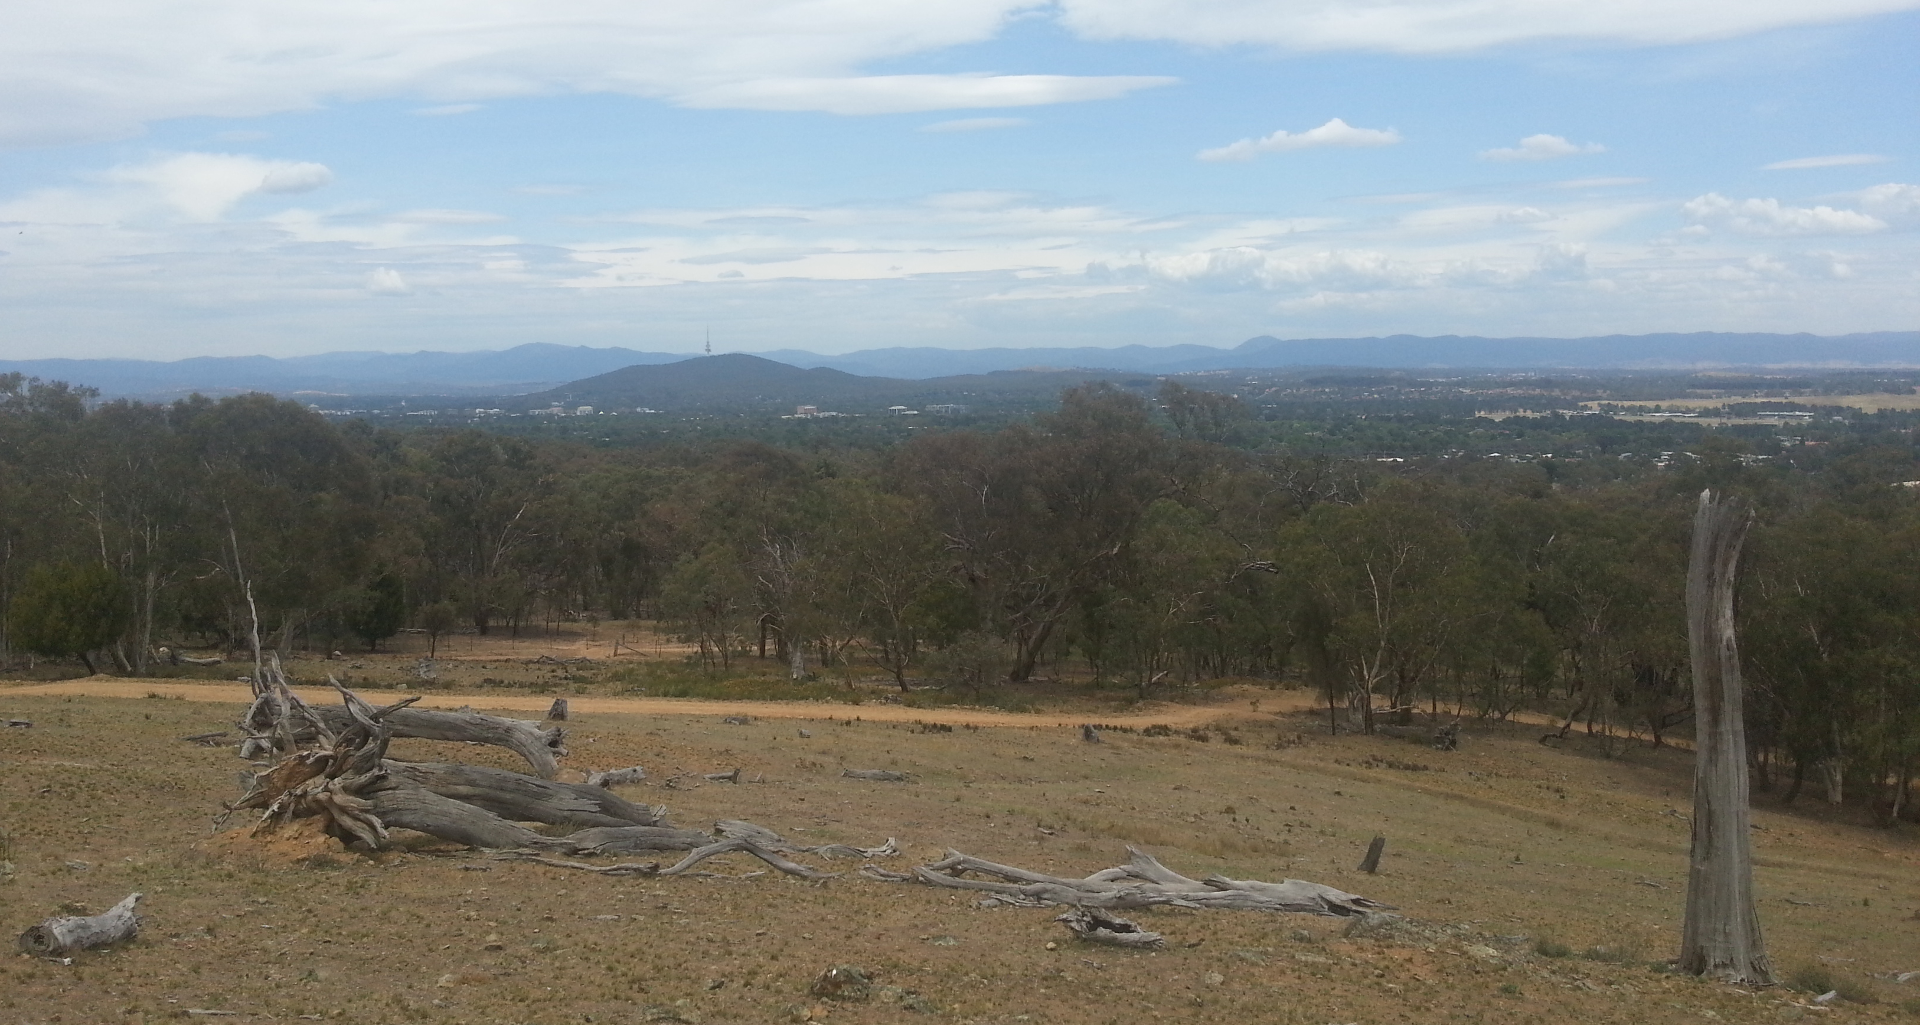
\includegraphics[width=0.8\textwidth]{img/canberra.png}
  \end{center}
\end{frame}

% \begin{frame}{Overview}
%   \begin{itemize}
%     \item Motivation
%     \item Technological overview
%     \item Early results and plans
%     \item Demonstration
%   \end{itemize}
% \end{frame}

\begin{frame}{Large-scale population genomics}
  \begin{itemize}
    \item Moving from 100s to 1,000s or 10,000s of samples \emph{per study!}
    \item Efficient algorithms to analyse large-scale genomic data
    \begin{itemize}
      \item Reference \& alignment free: \textit{less bias, de novo}
      \item Platform/protocol agnostic: \textit{future proof}
      \item Computationally efficient: \textit{not the bottleneck}
    \end{itemize}
  \end{itemize}
  \begin{center}
    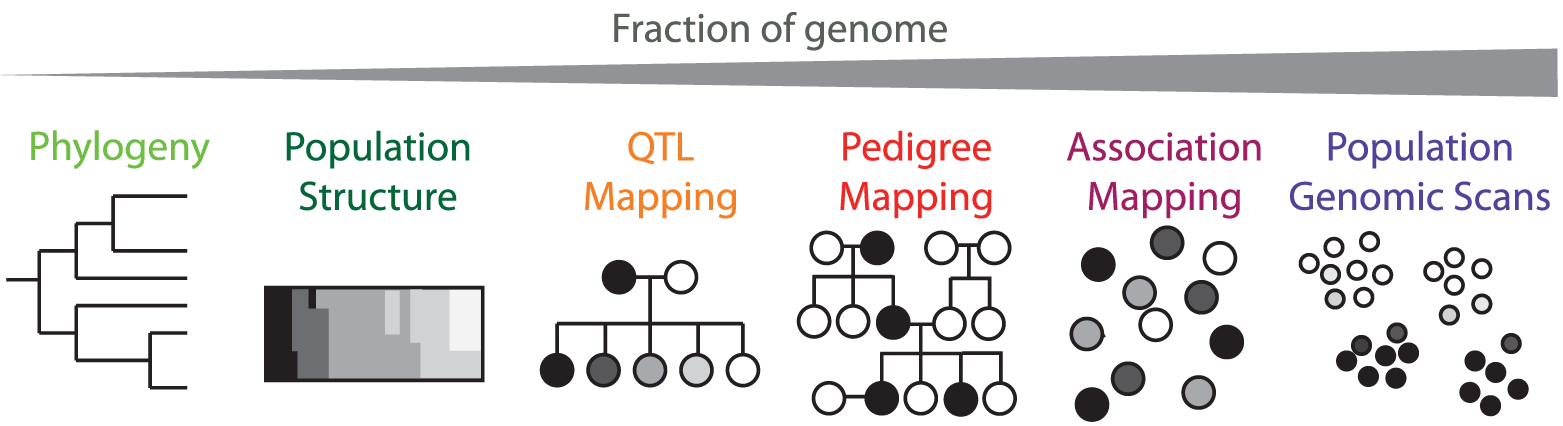
\includegraphics[width=\textwidth]{img/cross-scale.png}
  \end{center}
  \tiny{after \textcite{peterson_double_2012}}
\end{frame}



\begin{frame}{Genetic Similarity Estimation}
  \begin{itemize}
    \item Rough approximation of sample relatedness required
      \begin{itemize}
        \item For natural collections
        \item As a technical control
      \end{itemize}
  \end{itemize}
  \begin{center}
    \includegraphics<1>[width=\textwidth]{img/restruct-1}
    \includegraphics<2>[width=\textwidth]{img/restruct-2}
    \includegraphics<3>[width=\textwidth]{img/restruct-3}
    \begin{itemize}
      \item[]<1-3> \tiny{after \textcite{brachi_genome-wide_2011}}
    \end{itemize}
  \end{center}
\end{frame}

\begin{frame}[fragile]{\textit{De novo} technical control}
  \begin{itemize}
    \item Sample DNA not very physically distinctive
    \item Mislabeling, Misidentification, Contamination
  \end{itemize}
  \begin{center}
    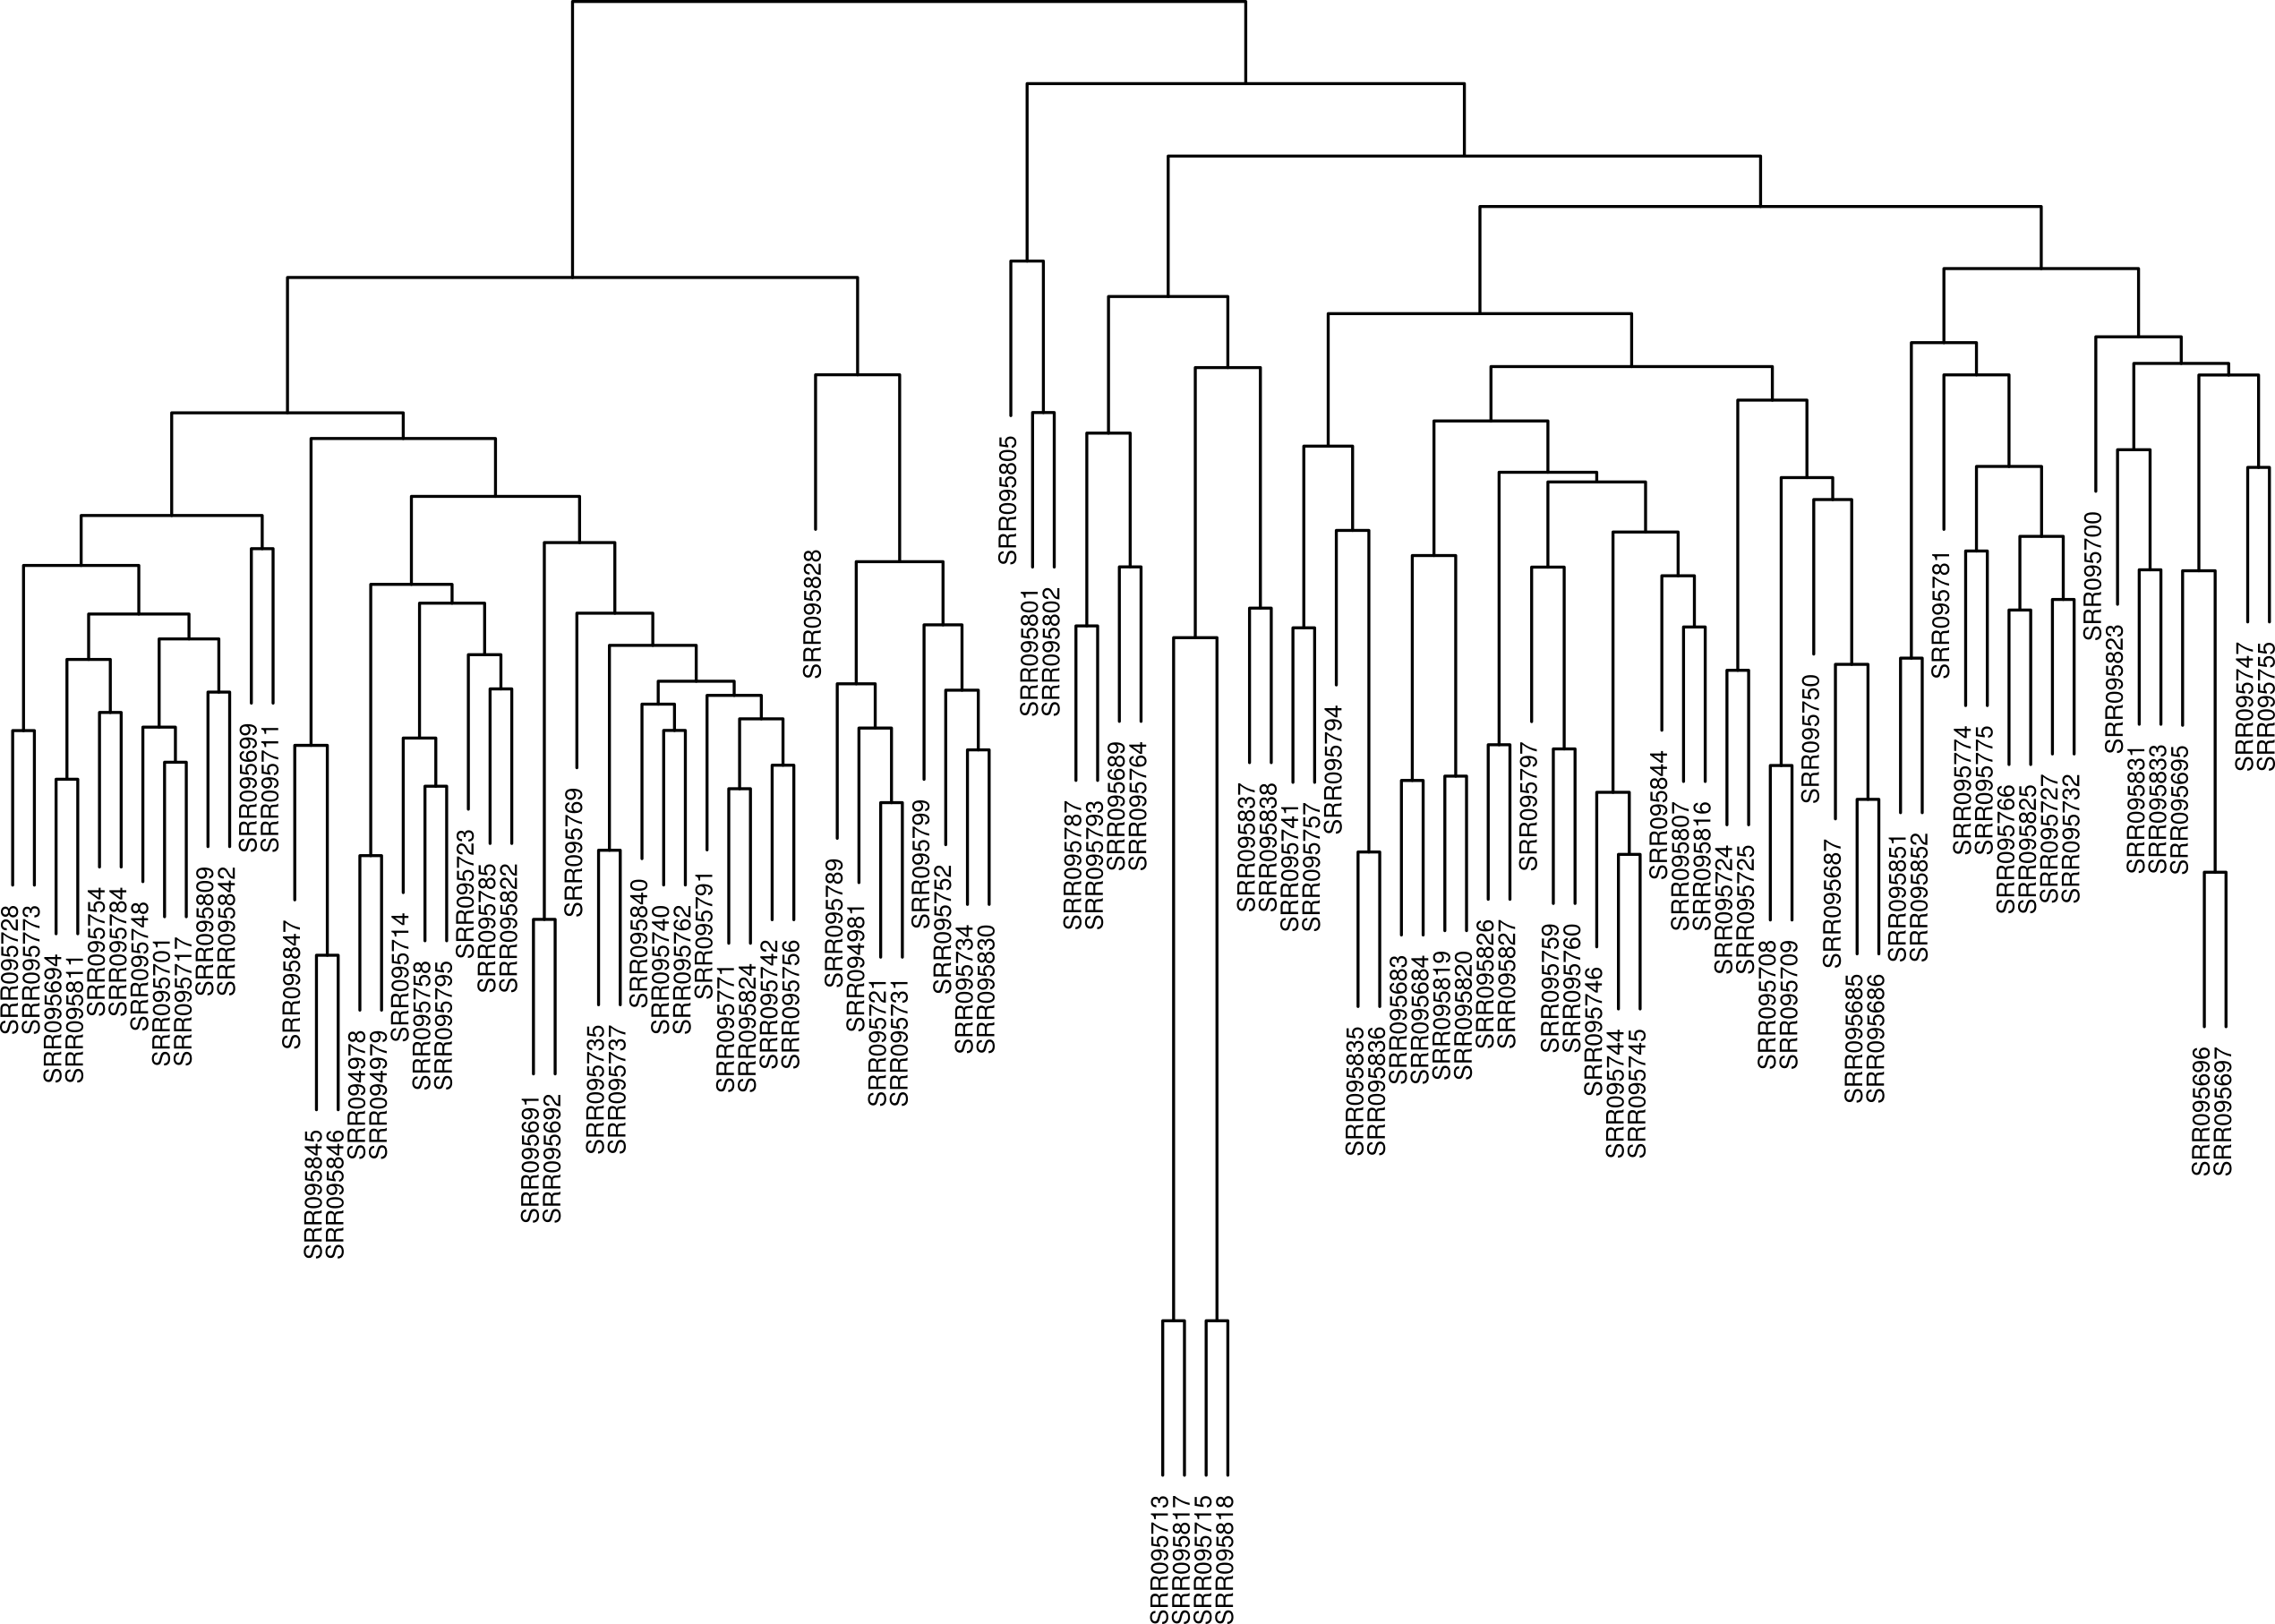
\includegraphics[width=0.6\textwidth]{img/at80-tree.png}
  \end{center}
  \pause
  \begin{center}
    \begingroup
      \fontsize{7pt}{7pt}\selectfont
      \begin{verbatim}
        54da64f0343b69bcb959d33f127505d8 SRR095713.fastq
        54da64f0343b69bcb959d33f127505d8 SRR095817.fastq
        7d74f1b53174afc9fd3aec1dde1d996e SRR095715.fastq
        7d74f1b53174afc9fd3aec1dde1d996e SRR095818.fastq
      \end{verbatim}
    \endgroup
  \end{center}
\end{frame}

\begin{frame}[c]{Genetic Similarity Estimation}
  \centering In many cases, we care mostly about the deepest and shallowest
  branches of the tree.
\end{frame}

\begin{frame}{Genetic Similarity Estimation}
  \begin{itemize}
    \item Which groups are my samples in?
    \item Which samples can be collapsed?
  \end{itemize}
  \begin{center}
    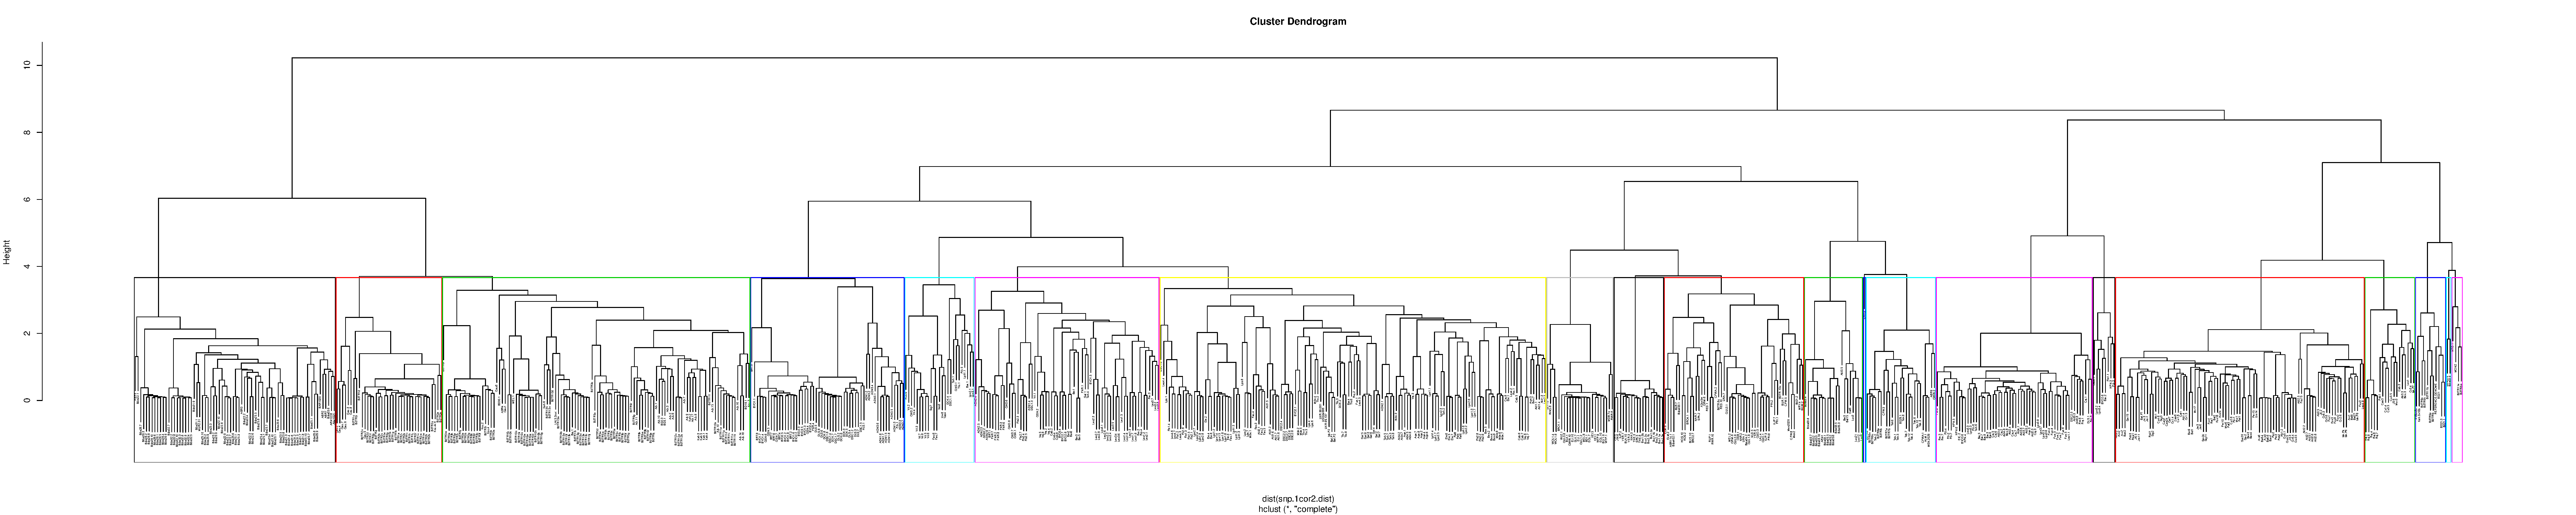
\includegraphics[width=\textwidth]{img/jared-tree.pdf}
  \end{center}
\end{frame}

\begin{frame}{Presenting \texttt{kWIP}}
  \begin{itemize}
    \item $k$-mer based \textit{de novo} genetic relatedness estimator
    \item Weighted Inner Product between hashes to determine relatedness
    \item Produces a distance matrix from raw NGS reads
  \end{itemize}
  \begin{center}
    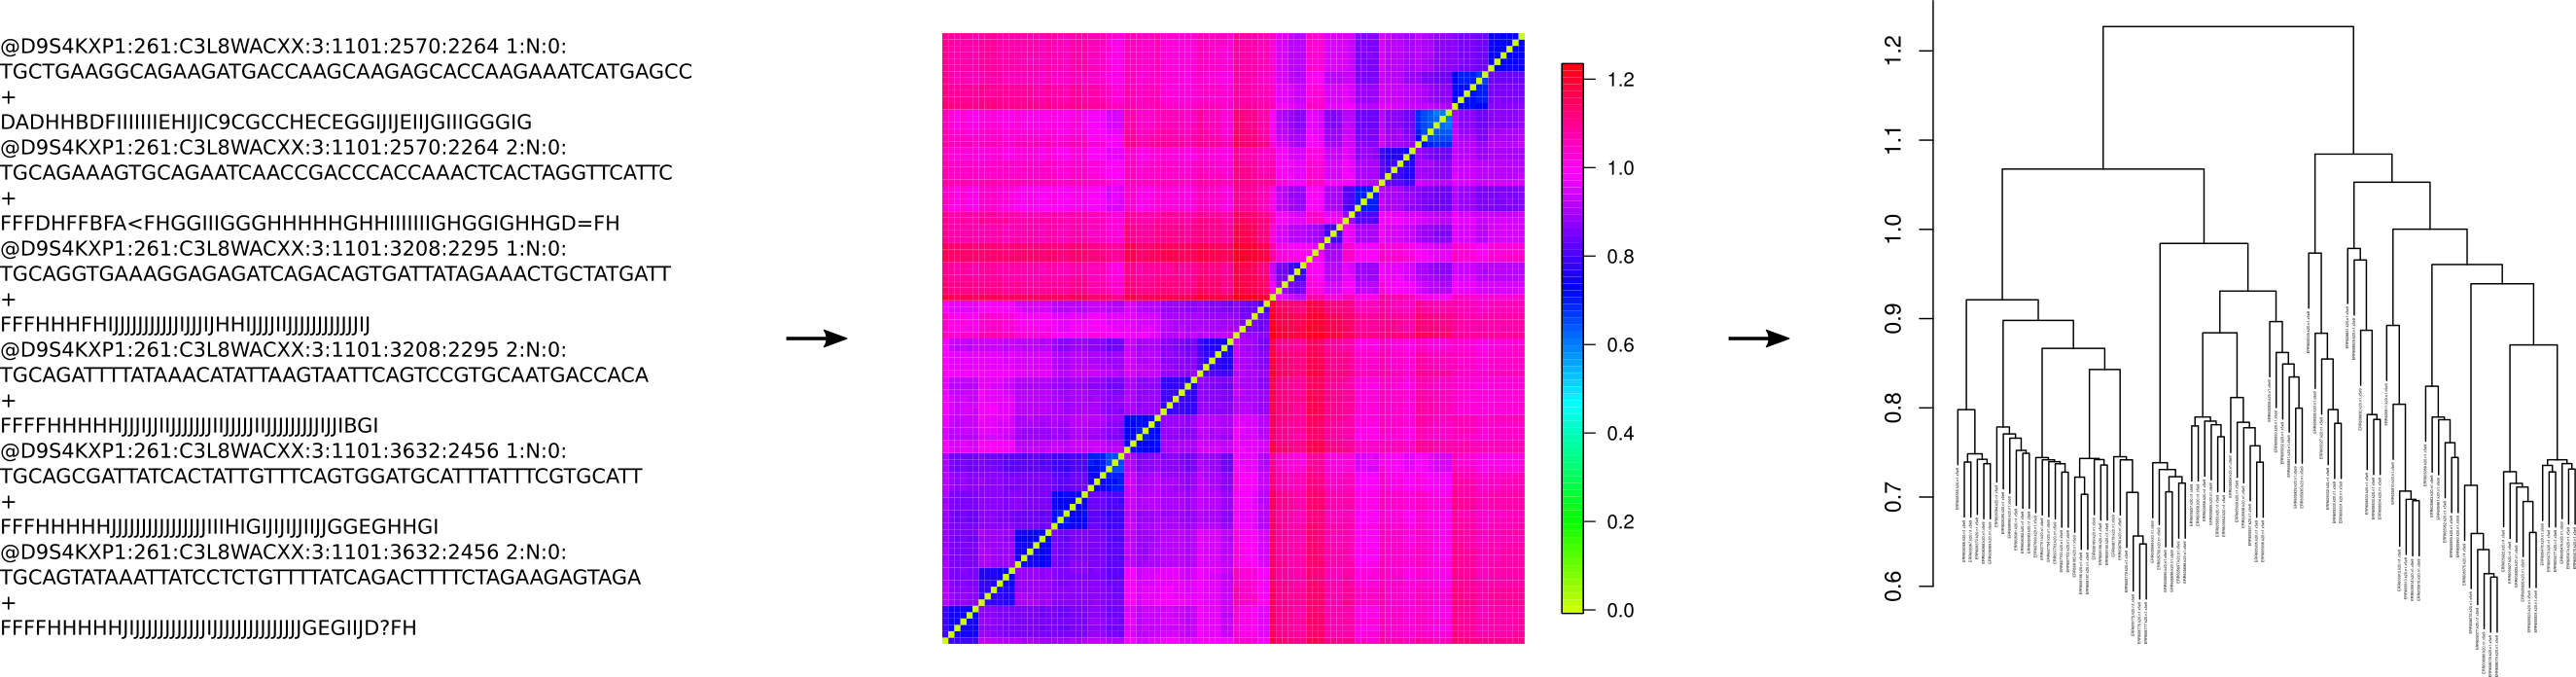
\includegraphics[width=\textwidth]{img/kwip-overview.png}
  \end{center}
\end{frame}

\begin{frame}{Technological Overview}
  \begin{itemize}
    \item Alignment-free Sequence Comparison
    \item Hashing and Probabilistic Data Structures
    \item Population and Frequency Hashes
    \item (Weighted) Inner Products
  \end{itemize}
\end{frame}

\begin{frame}{$k$-mer Seq. Comparison}
  \begin{columns}[t]
    \column{0.5\textwidth}
      \begin{itemize}
        \item<1-> Analyse sequences by decomposition to $k$-length words
        \item<1-> Computationally and biologically appropriate
        \begin{itemize}
          \item<1-> Fast: Scalable and parallelisable
          \item<1-> Constant-memory (using \texttt{khmer})
          \item<1-> Reference-free
          \item<1-> Easily scales to longer or more reads \end{itemize} \end{itemize}
    \column{0.5\textwidth}
    \begin{center}
      \includegraphics<1>[height=0.6\textheight]{img/ali.png}
      \includegraphics<2>[height=0.6\textheight]{img/ali-free.png}
    \end{center}
  \end{columns}
\end{frame}

\begin{frame}{$k$-mer Seq. Comparison}
  \begin{itemize}
    \item Many existing tools
    \begin{itemize}
      \item Feature Frequency Profiles \autocite{sims_alignment-free_2009}
      \item $D2$ and related statistics
      \item \texttt{spaced} and other spaced-word approaches
        \autocite{morgenstern_estimating_2015,leimeister_fast_2014}
      \item Early steps in BLAST \textit{et al.}
    \end{itemize}
    \item Most require assembled gene/genome sequence
    \item Many use inner product as similarity measure
  \end{itemize}
\end{frame}


\begin{frame}{Hashes and Hash Functions}
  \begin{itemize}
    \item ``Hash'': a probabilistic data structure
      \begin{itemize}
        \item Efficient way of counting k-mers
        \item Constant memory
        \item Easy set operations and inner product
        \item Implicit de Bruijn graph
        \item Implemented in Titus Brown's \texttt{khmer}
      \end{itemize}
    \item Hash function
      \begin{itemize}
        \item Function over bytes $=>$ number
        \item e.g.: \mint{python}|hash('ACG') => 5234315134| \texttt{md5sum}
        \item For DNA, 2-bit encoding is common for $k \le  32$
      \end{itemize}
  \end{itemize}
\end{frame}

\begin{frame}{Hash}
  \begin{itemize}
    \item Subset of a Count-Min Sketch/Counting Bloom Filter
    \item Vector of large prime length (e.g. 1e9 + 7)
    \item Indexed modulo length $(bin = h(w_i) \mod prime)$
    \item Aliasing can occur, hence probabilistic
  \end{itemize}
  \begin{center}
    \includegraphics<1>[width=0.6\textwidth]{img/hash-0.png}
    \includegraphics<2>[width=0.6\textwidth]{img/hash-1.png}
    \includegraphics<3>[width=0.6\textwidth]{img/hash-2.png}
    \includegraphics<4>[width=0.6\textwidth]{img/hash-3.png}
    \includegraphics<5>[width=0.6\textwidth]{img/hash-4.png}
  \end{center}
\end{frame}


\begin{frame}{Hash Operations}
  \begin{itemize}
    \item Population sum, or hash frequency
  \end{itemize}
  \begin{center}
    \includegraphics<1>[width=0.6\textwidth]{img/hash-sums.png}
    \includegraphics<2>[width=0.6\textwidth]{img/hash-sumfreq.png}
  \end{center}
  \begin{itemize}
    \item<2-> Many more efficient operations \small{(union, intersect etc.)}
  \end{itemize}
\end{frame}

\begin{frame}{Entropy Weighting}
  \begin{itemize}
    \item \texttt{kWIP} weights by Shannon entropy: $H(frequency)$
    \item Shannon entropy: measure of information
    \item $ -\sum\limits_{i} p_i log(p_i) $
  \end{itemize}
  \begin{center}
    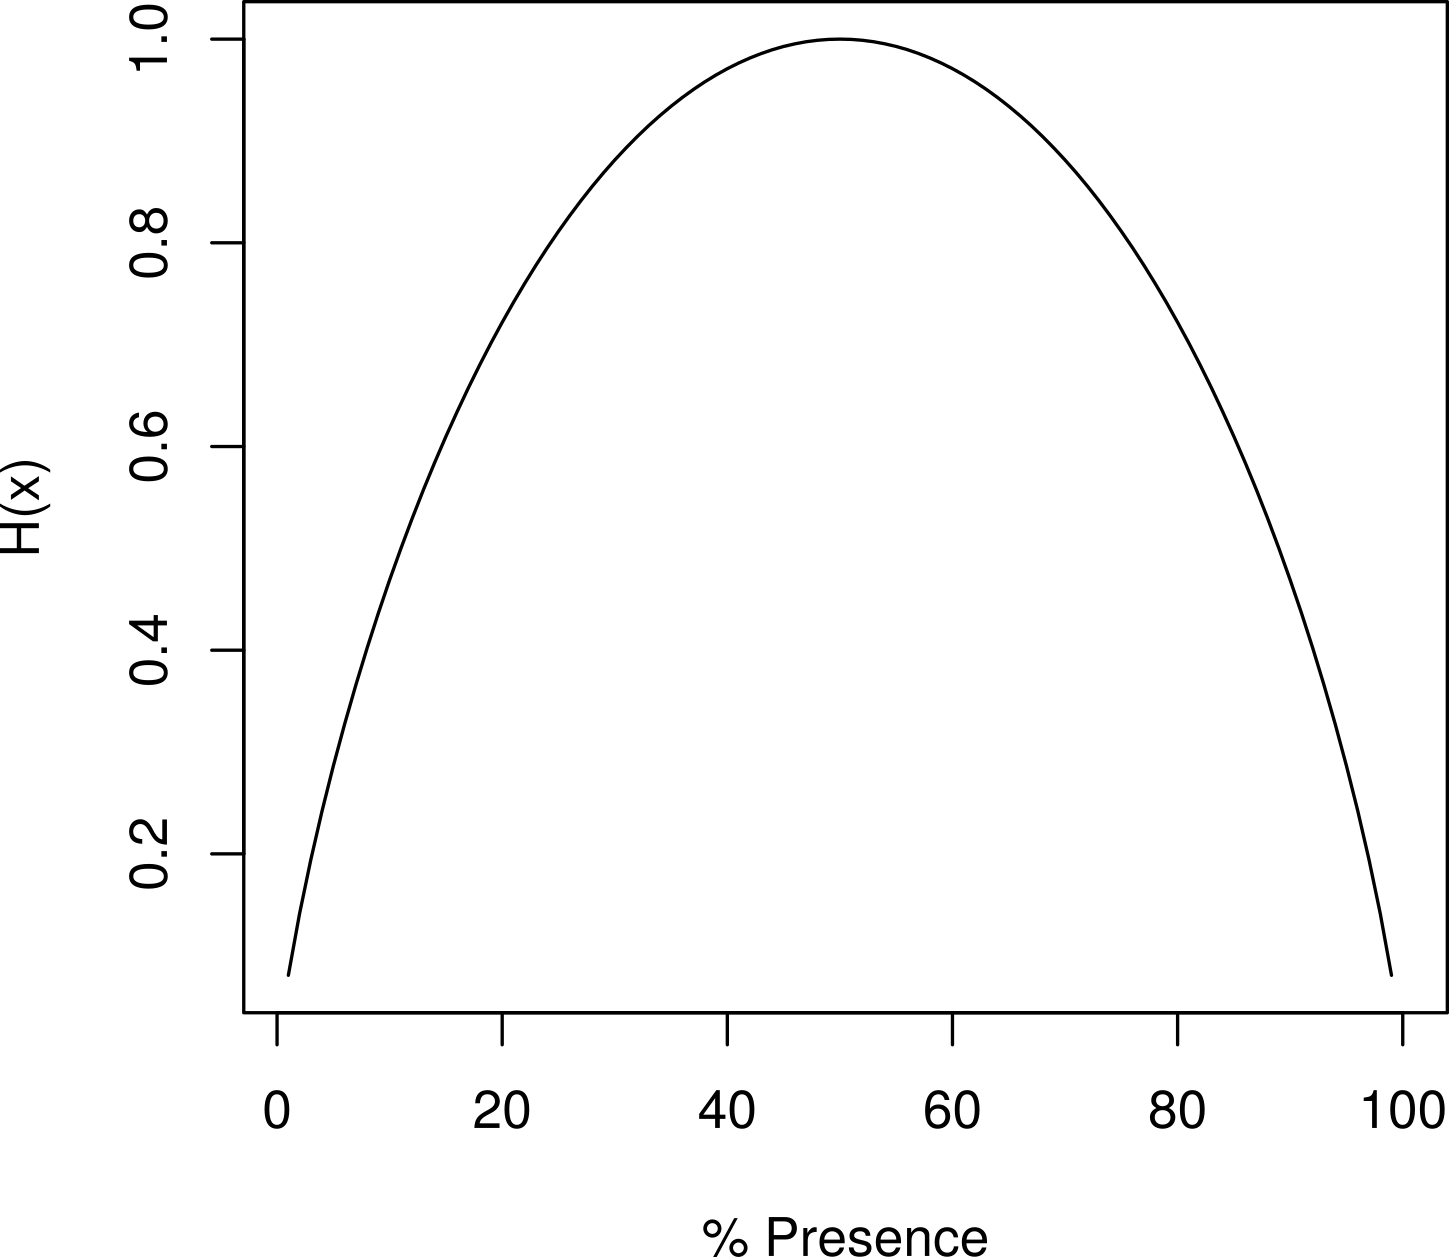
\includegraphics[width=0.6\textwidth]{img/shanent.png}
  \end{center}
\end{frame}

\begin{frame}{Side note: Terminology}
  \begin{columns}
    \begin{column}{0.6\textwidth}
      \begin{itemize}
        \item Sample: a biological thing, e.g plant, leaf, mouse foot.
        \item Run: The set of reads resulting form one sequencing library from
          a single sample
        \item May be $>1$ run per sample, strictly 1 sample per run
      \end{itemize}
    \end{column}
    \begin{column}{0.4\textwidth}
      \begin{center}
        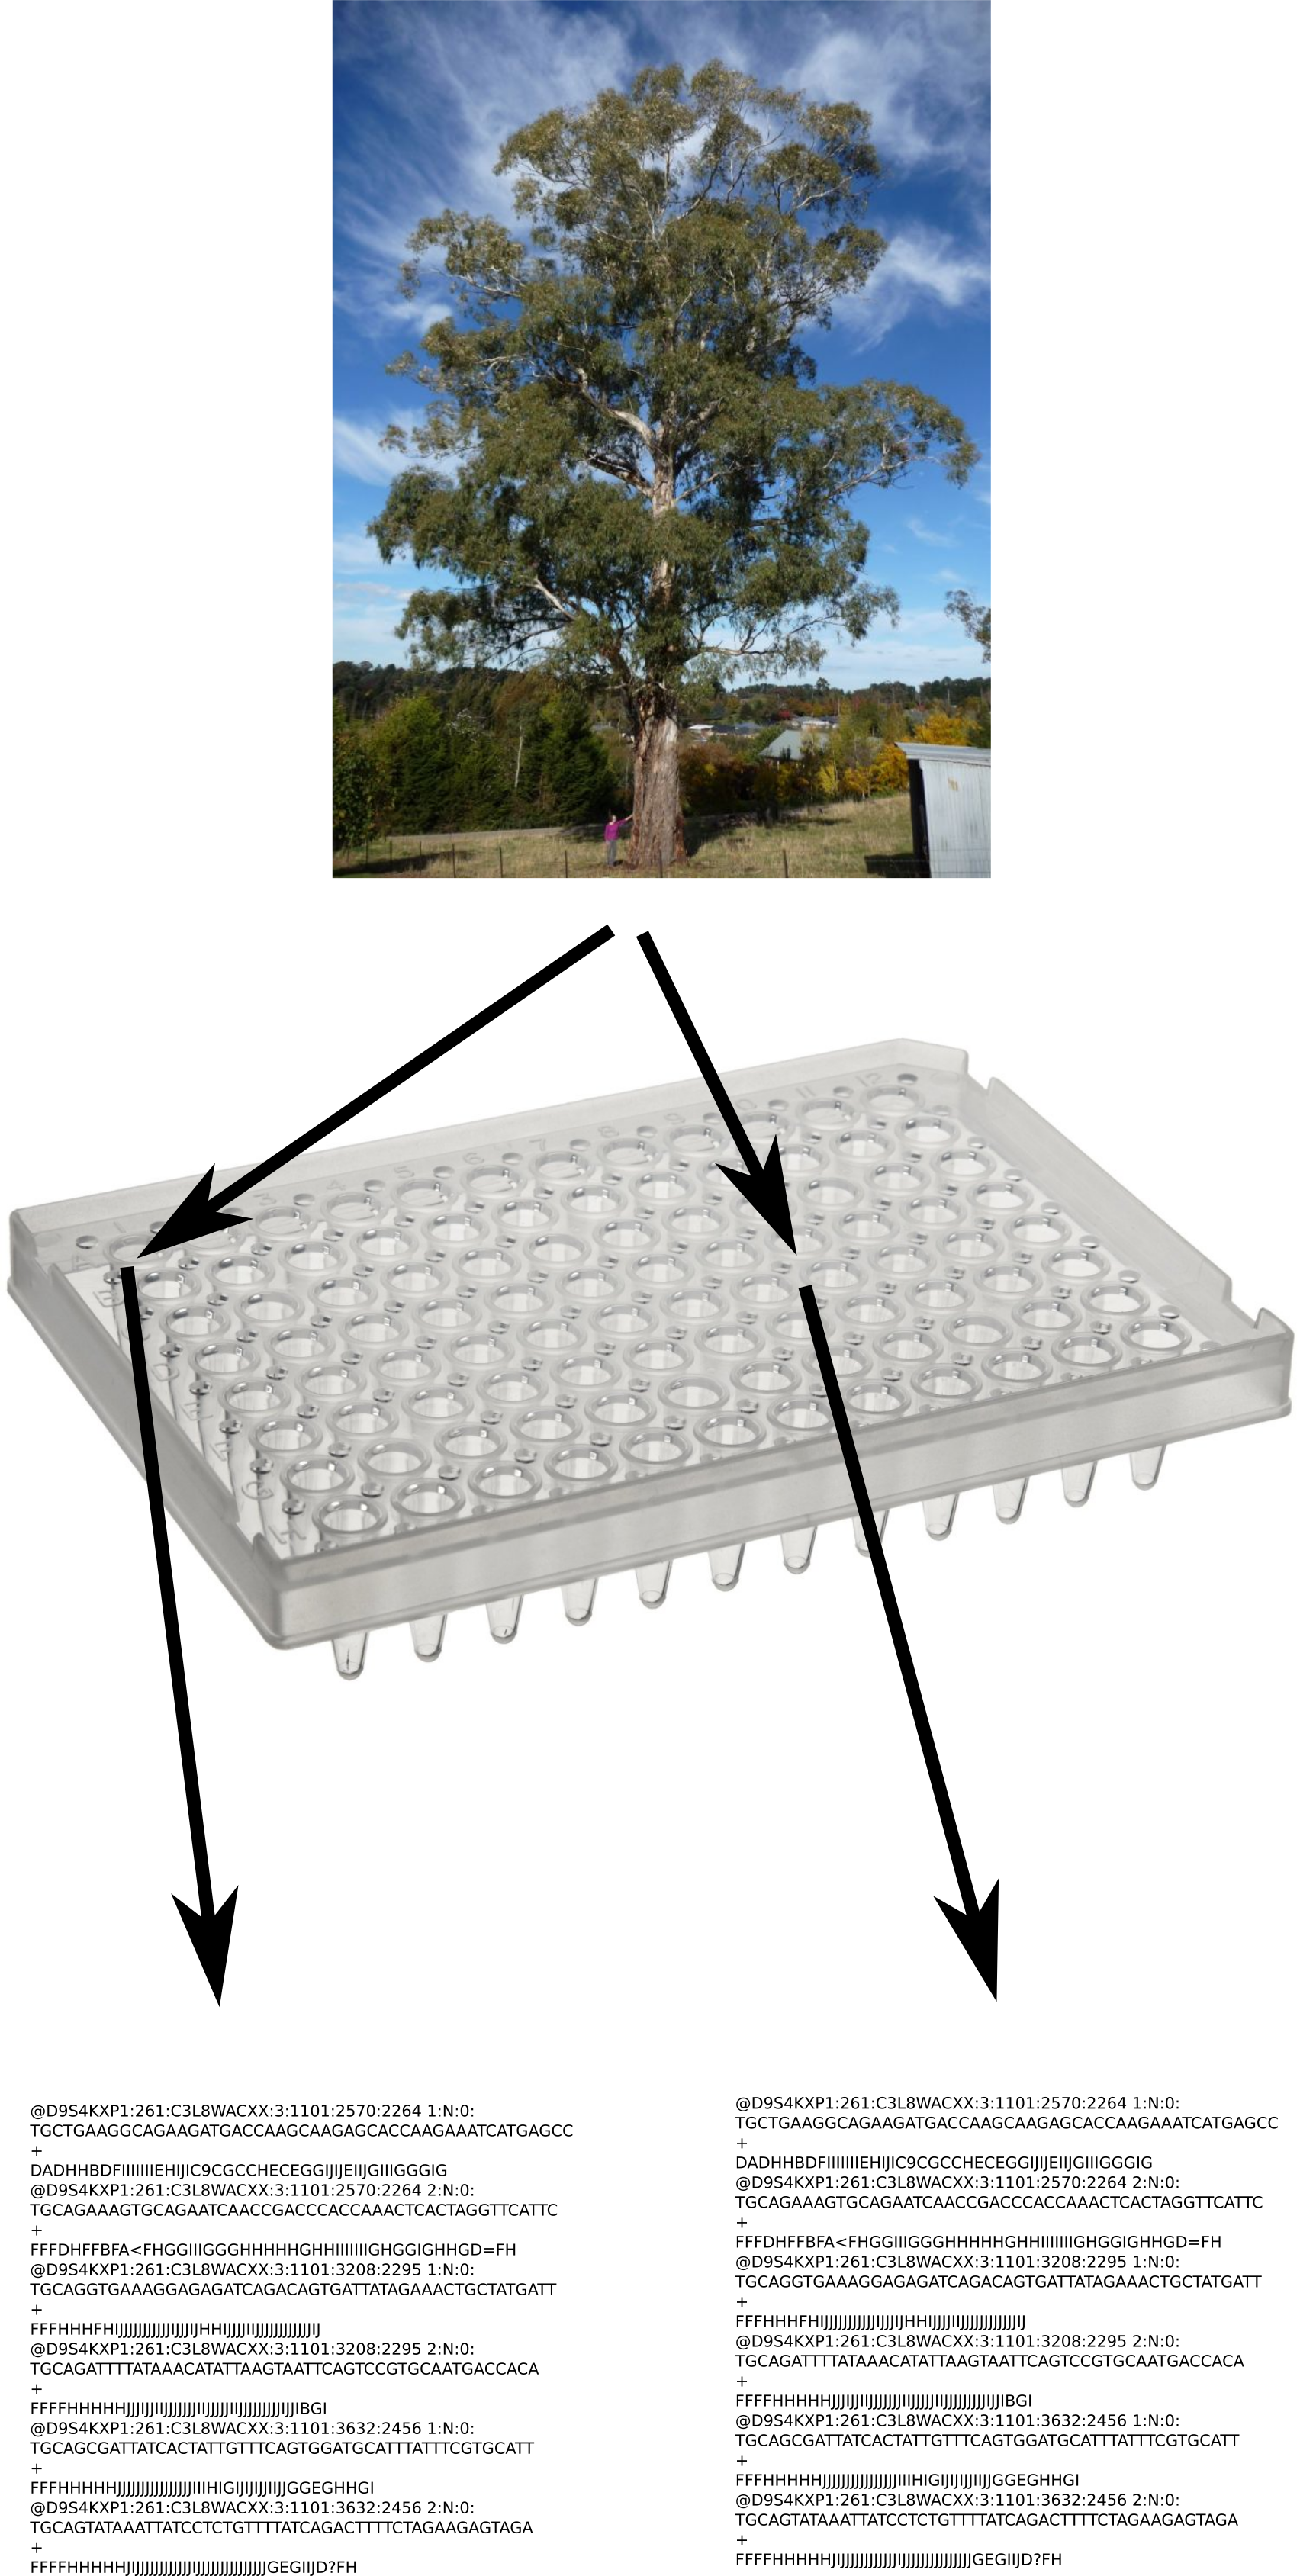
\includegraphics[width=0.6\textwidth]{img/sample-run.png}
      \end{center}
    \end{column}
  \end{columns}
\end{frame}

\begin{frame}{\texttt{kWIP} Algorithm}
  \begin{itemize}
    \item For each run: count all $k$-mers into a hash
    \pause
    \item For each analysis set, i.e ``population'':
      \begin{itemize}
        \item Calculate the entropy of population frequency ($H$)
        \item For each pair of runs $A$ and $B$, calculate \\
          $\sum\limits^{n}_{i=0} A_i \cdot B_i \cdot H_i$
      \end{itemize}
  \end{itemize}
  \begin{center}
    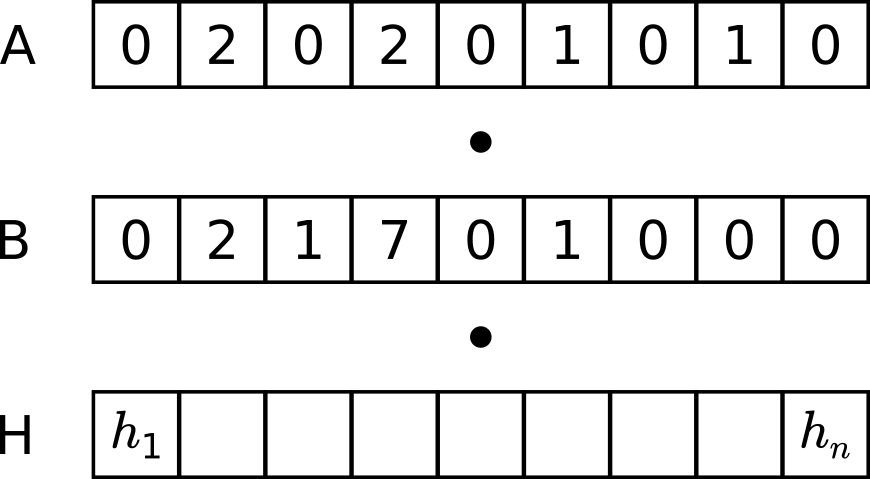
\includegraphics[width=0.4\textwidth]{img/hash-wip.png}
  \end{center}
\end{frame}


\begin{frame}{\texttt{kWIP}}
  \begin{itemize}
    \item The software:
      \begin{itemize}
        \item \texttt{C++}, $>$2000 lines of code
        \item Uses \texttt{khmer} for $k$-mer counting \& hashing
        \item Parallelised, fast
        \item GNU GPL licensed, source code on GitHub
      \end{itemize}
      \begin{center}
        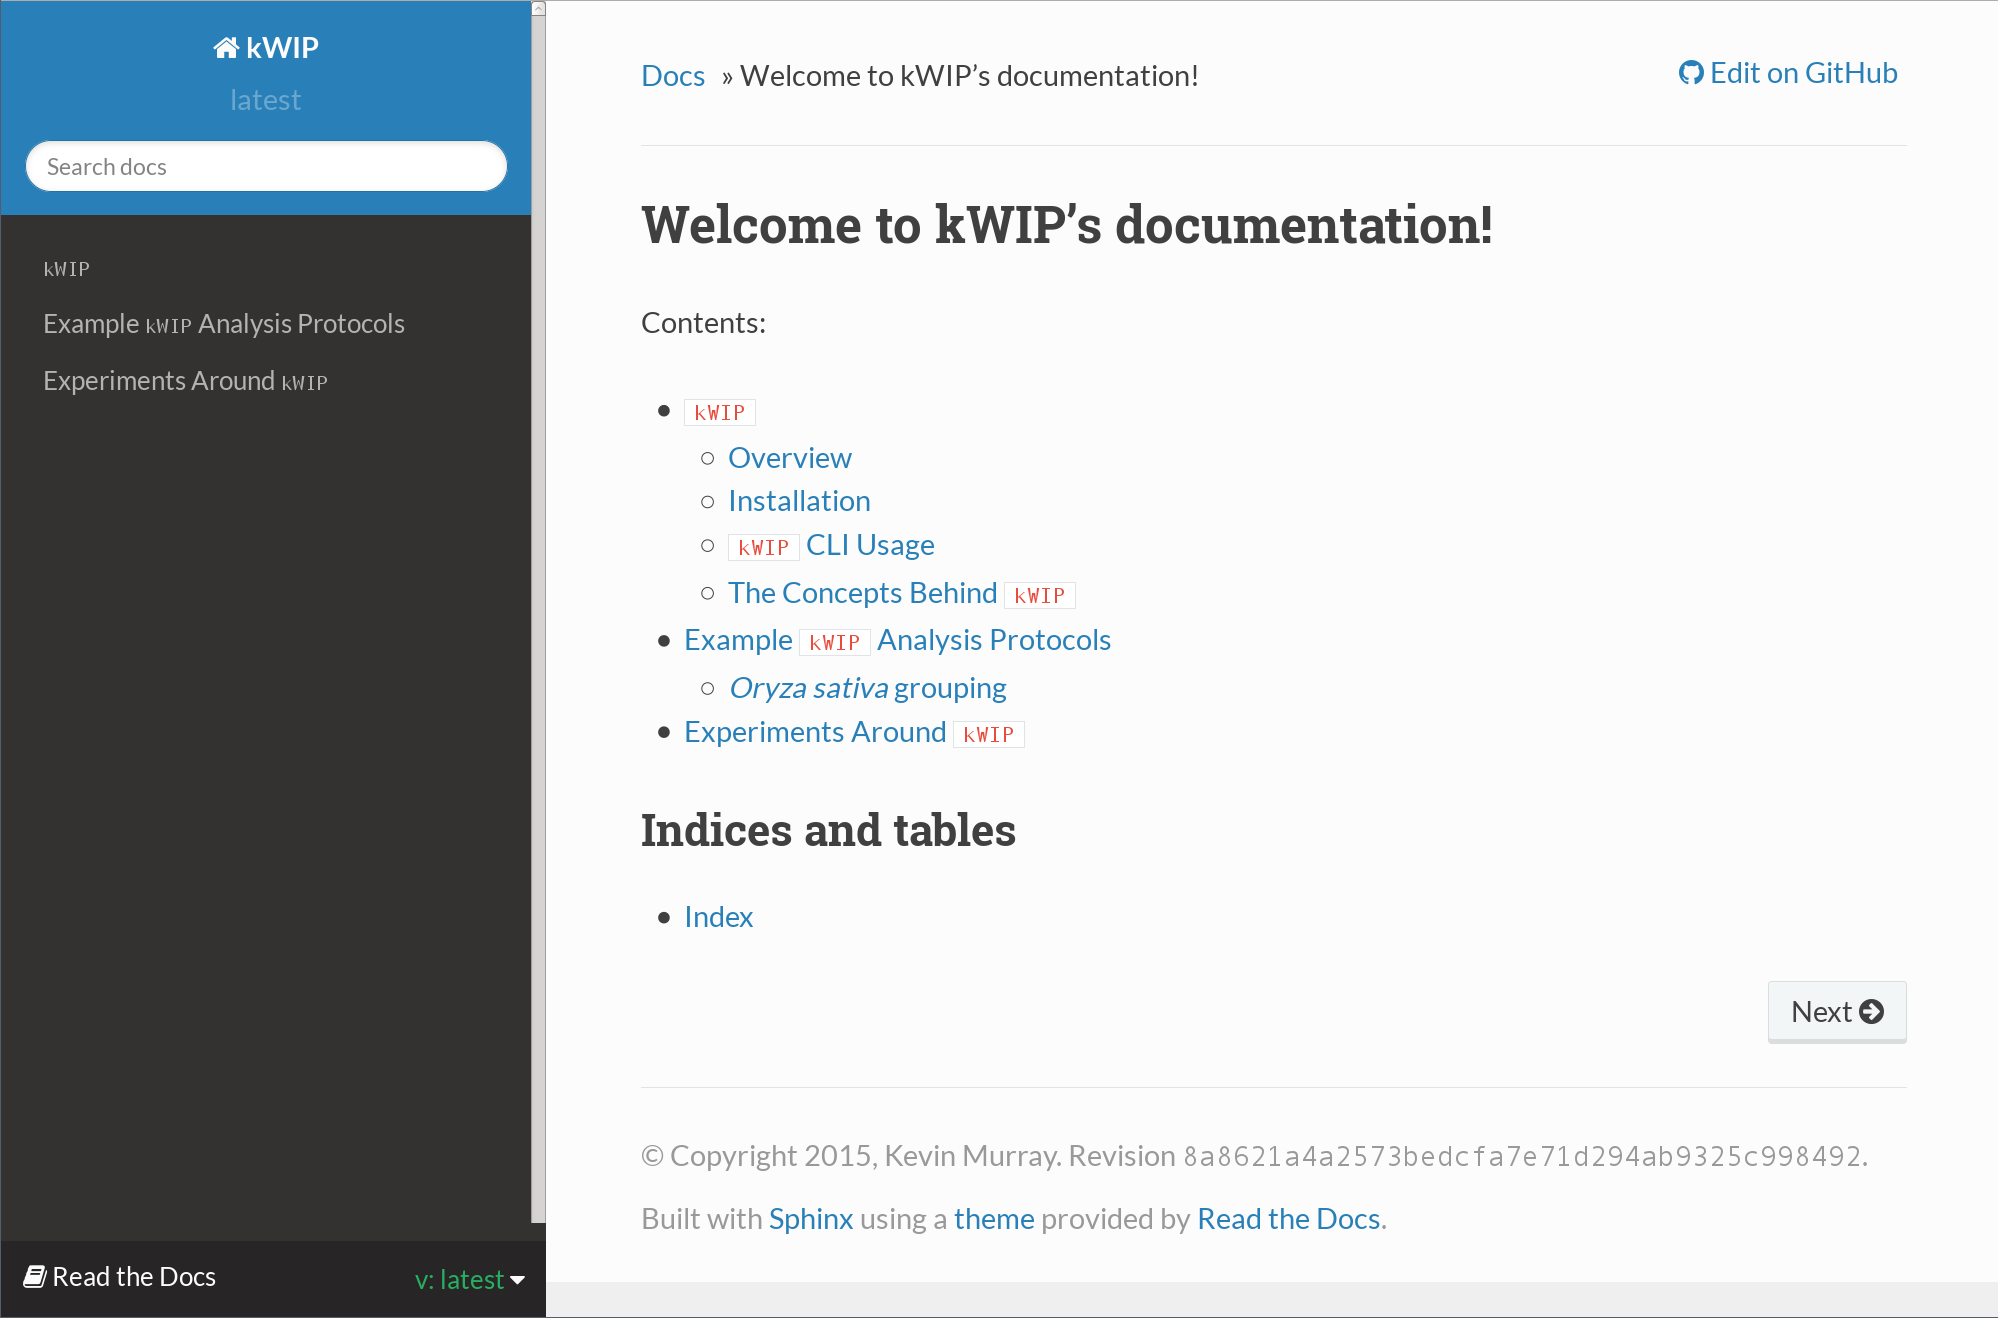
\includegraphics[width=0.5\textwidth]{img/kwip-doc-screenshot.png}
      \end{center}
  \end{itemize}
\end{frame}

\begin{frame}{\texttt{kWIP} Case Studies}
  \begin{itemize}
    \item 3000 rice genomes:
      \begin{itemize}
        \item 3000 rice samples (25k runs)
          \autocite{the_3000_rice_genomes_project_3000_2014}
        \item Analysing in sets of 96, from all major groups
      \end{itemize}
    \item Chlamydomonas
      \begin{itemize}
        \item $\approx 20$ lines from USA
        \item High coverage re-sequencing with leftover assembly
        \item Compare to SNP-based distance calculation
      \end{itemize}
    \item Simulation
      \begin{itemize}
        \item Fake population genome sequencing studies
      \end{itemize}
  \end{itemize}
\end{frame}

\begin{frame}{96 Rice Runs}
  \begin{itemize}
    \item Set of 96 rice runs from 16 samples (6 tech reps ea)
    \item About half/half from 2 major groups (Indica, Japonica)
    \item Expectations:
      \begin{itemize}
        \item All runs cluster into groups of 6 reps (16 samples)
        \item Big split between two groups: (7 and 9 respectively here)
      \end{itemize}
    \item Recover known grouping w/ \texttt{kWIP}, not w/ unweighted IP
    \item Sensitive to read depth
    \item Took $\approx 10$ hours on 16 CPU, 84GB RAM supercomputer node
  \end{itemize}
\end{frame}

\begin{frame}
  \begin{center}
    \includegraphics<1>[width=\textwidth]{img/distmat-both.png}
    \includegraphics<2>[width=\textwidth]{img/dendro-both.png}
  \end{center}
\end{frame}

\begin{frame}
  \begin{center}
    \includegraphics<1>[width=0.6\textwidth]{img/dendro-wip.png}
    \includegraphics<2>[width=0.6\textwidth]{img/dendro-ip.png}
  \end{center}
\end{frame}

\begin{frame}{Chlamydomonas}
  \begin{center}
    \includegraphics<1>[width=0.6\textwidth]{img/chlamydomonas_PCA_from_paper.png}
    \includegraphics<2>[width=0.6\textwidth]{img/chlamydomonas_PCA_full-set-dim_1-3.png}
    \begin{itemize}
      \item Population genomics of Chlamy in USA
      \item[] \tiny{Data from \textcite{flowers_whole-genome_2015}}
    \end{itemize}
  \end{center}
\end{frame}

\begin{frame}{Simulation}
  \begin{itemize}
    \item Perform simulated sequencing experiment:
    \begin{itemize}
      \item Simuate natural population structure
      \item Simulate sample genomes, sequencing runs
      \item Hash reads, kWIP
    \end{itemize}
    \item kWIP quantitatively better than unweighted equivalent
  \end{itemize}
  \begin{center}
    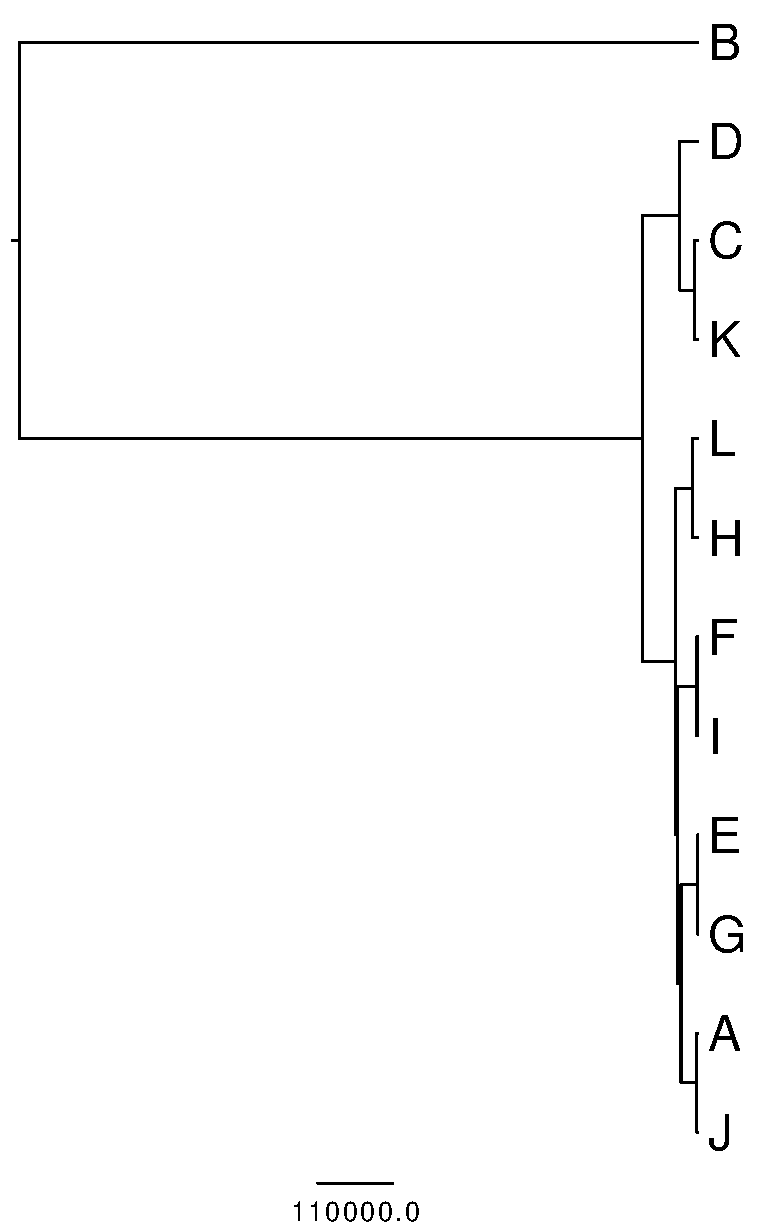
\includegraphics[width=0.3\textwidth]{img/sampletree.pdf}
  \end{center}
\end{frame}

\begin{frame}
  \begin{center}
    \includegraphics<1>[width=\textwidth]{img/Truth-mat.png}
    \includegraphics<2>[width=\textwidth]{img/WIP-mat.png}
    \includegraphics<3>[width=\textwidth]{img/IP-mat.png}
    \includegraphics<4>[width=\textwidth]{img/WIPvsIPvsTruth.png}
    \begin{itemize}
      \item[] <4> WIP $\rho = 0.95$, IP $\rho = 0.86$
    \end{itemize}
  \end{center}
\end{frame}

\begin{frame}{Conclusions}
  \begin{itemize}
    \item \texttt{kWIP} is implemented, Beta software
    \item Publically available at \url{github.com/kdmurray91/kwip}
    \item We show the utility of \texttt{kWIP}
    \item Publication coming soon
    \pause
    \item What's next?
      \begin{itemize}
        \item Norman will lead the kWIP project's evolution
        \item I will focus on assembly
      \end{itemize}
  \end{itemize}
\end{frame}

\begin{frame}{Thanks}
  \begin{itemize}
    \item My collaborators
      \begin{itemize}
        \item Cheng Soon Ong
        \item Christfried Webers
        \item Norman Warthmann
        \item Sylvain For\^{e}t
      \end{itemize}
    \item Supervisors:
      \begin{itemize}
        \item Justin Borevitz
        \item Gavin Huttley
        \item Barry Pogson
      \end{itemize}
    \item \texttt{khmer} folks (DIB-lab, UC Davis)
      \begin{itemize}
        \item C. Titus Brown
        \item Michael Crusoe
        \item Camille Scott
      \end{itemize}
    \item Yourselves
  \end{itemize}
\end{frame}

\begin{frame}[shrink=20]{}
  \printbibliography
  \vfill
  .
\end{frame}

\end{document}
